\documentclass[fleqn, a4paper, 12pt, twoside]{article}
\usepackage{exsheets} %question and solution environments
\usepackage{amsmath, amssymb, amsthm} %standard AMS packages
\usepackage{esint} %integral signs
\usepackage{marginnote} %marginnotes
\usepackage{gensymb} %miscellaneous symbols
\usepackage{commath} %differential symbols
\usepackage{xcolor} %colours
\usepackage{cancel} %cancelling terms
\usepackage{siunitx} %formatting units
\usepackage{tikz, pgfplots} %diagrams
	\usetikzlibrary{calc, hobby, patterns, intersections, angles, quotes}
\usepackage{graphicx} %inserting graphics
\usepackage{epstopdf} %converting and inserting eps graphics
\usepackage{hyperref} %hyperlinks
\usepackage{datetime} %date and time
\usepackage{ulem} %underline for \emph{}
\usepackage{xfrac, lmodern} %inline fractions
\usepackage{enumerate} %numbered lists
\usepackage{float} %inserting floats
\usepackage{circuitikz} %circuit diagrams

\newcommand\numberthis{\addtocounter{equation}{1}\tag{\theequation}} %adds numbers to specific equations in non-numbered list of equations

\newcommand{\AxisRotator}[1][rotate=0]{
	\tikz [x=0.25cm,y=0.60cm,line width=.2ex,-stealth,#1] \draw (0,0) arc (-150:150:1 and 1);%
} %rotation symbols on axes

\theoremstyle{definition}
\newtheorem{example}{Example}
\newtheorem{definition}{Definition}

\theoremstyle{theorem}
\newtheorem{theorem}{Theorem}
\newtheorem{law}{Law}

\newcommand{\curl}{\mathrm{curl\,}}

\newcommand{\divergence}{\mathrm{div\,}}

\makeatletter
\@addtoreset{section}{part} %resets section numbers in new part
\makeatother

\newcommand\blfootnote[1]{%
	\begingroup
	\renewcommand\thefootnote{}\footnote{#1}%
	\addtocounter{footnote}{-1}%
	\endgroup
}

\SetupExSheets{solution/print = true} %prints all solutions by default

%opening
\title{Physics 2}
\author{Aakash Jog}
\date{2014-15}

\begin{document}

\maketitle
%\setlength{\mathindent}{0pt}

\blfootnote
{	
	\begin{figure}[H]
		
\includegraphics[height = 12pt]{cc.eps}
		\includegraphics[height = 12pt]{by.eps}
		\includegraphics[height = 12pt]{nc.eps}
		\includegraphics[height = 12pt]{sa.eps}
	\end{figure}
	This work is licensed under the Creative Commons Attribution-NonCommercial-ShareAlike 4.0 International License. To view a copy of this license, visit \url{http://creativecommons.org/licenses/by-nc-sa/4.0/}.
} %CC-BY-NC-SA license

\tableofcontents

\newpage
\section{Lecturer Information}

\textbf{Dr. Erez Pyetan}\\
~\\
Office: Sharet 325\\
Telephone: 7565\\
E-mail: erezpyet@mail.tau.ac.il\\

\section{Textbooks}

\begin{enumerate}
	\item D. Halliday, R. Resnick, and K. S. Krane: \textit{Physics}, 5th edition, vol. 2 (Wiley)
	\item D.J. Griffiths: \textit{Introduction to Electrodynamics}
\end{enumerate}

\newpage
\part{Electrostatics}

\section{Coulomb's Law}

\begin{law}[Coulomb's Law]
	The force between two charged particles is directly proportional to the product of the charges of the particles, and inversely proportional to the square of the distance between them.
	\begin{align*}
		F &\propto \dfrac{q_1 q_2}{r^2}\\
		F &= k \dfrac{q_1 q_2}{r^2}\\
		&= \dfrac{1}{4 \pi \varepsilon_0} \cdot \dfrac{q_1 q_2}{r^2}
	\end{align*}
	The constant of proportionality is $k = 8.99 \times 10^9 \si{\newton\metre\squared\per\coulomb\squared}$.\\
	$\varepsilon_0 = 8.8541878162 \times 10^{-12} \si{\coulomb\squared\per\newton\per\metre\squared}$ is called the permittivity of free space.\\
	In vector notation,
	\begin{align*}
		\overrightarrow{F_{2 1}} &= \dfrac{1}{4 \pi \varepsilon_0} \dfrac{q_1 q_2}{{r_{1 2}}^2} \hat{r_{1 2}}
	\end{align*}
\end{law}
~\\
Charge is defined according to this law.\\

\begin{question}
	A charge $q$ is placed at the origin. A charge $-2q$ is placed at 1 \si{\metre} from it, in the $x$ direction. Find a point on the $y$-axis where the total force acting on a charge $q'$ will be parallel to the $x$-axis.\\
\end{question}

\begin{solution}
	\begin{figure}[H]
		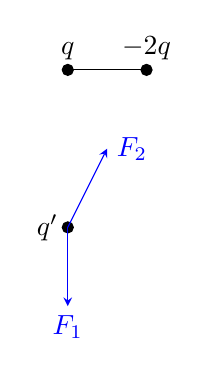
\begin{tikzpicture}
			\def\y{-2};
			\def\F{1};
			
			\coordinate (q) at (0,0);
			\coordinate (-2q) at (1,0);
			\coordinate (q') at (0,\y);
			
			\filldraw (q) circle [radius = 2pt] node [above] {$q$};
			\filldraw (-2q) circle [radius = 2pt] node [above] {$-2q$};
			\filldraw (q') circle [radius = 2pt] node [left] {$q'$};
			
			\draw (q) -- (-2q);
			
			\begin{scope}[blue, -stealth]
				\draw (q') -- ++(-90:\F) node [below] {$F_1$};
				\draw (q') -- ($ (q') ! 0.5 ! (-2q) $) node [right] {$F_2$};
			\end{scope}
		\end{tikzpicture}
	\end{figure}
	For the net force to be in the $x$ direction, the components of $F_1$ and $F_2$ in the $y$ direction must cancel each other out.
	\begin{align*}
		F_1 &= F_2 \sin \theta\\
		\therefore \cancel{k} \cdot \dfrac{(\cancel{q'})(-2\cancel{q})}{y^2 + 1} \cdot \dfrac{y}{\sqrt{y^2 + 1}} &= \cancel{k} \cdot \dfrac{(\cancel{q})(\cancel{q'})}{y^2}\\
		\therefore \dfrac{-2y}{(y^2 + 1)^{\sfrac{3}{2}}} &= \dfrac{1}{y^2}\\
		\therefore y &= \pm \sqrt{\dfrac{1}{2^{\sfrac{2}{3}}- 1}}
	\end{align*}
\end{solution}

\begin{question}
	A rod of length $L$ has a uniformly distributed charge $Q$, with line charge density $\lambda = \dfrac{Q}{L}$. A point charge $q$ is kept at a distance $x$ as shown.
	\begin{figure}[H]
		\begin{tikzpicture}
			\def\L{5};
			\def\x{10};
			
			\coordinate (q) at (\x,0);
			
			\draw [ultra thick] (0,\L/2) -- (0,-\L/2);
			
			\filldraw (q) circle [radius = 2pt] node [right] {$q$};
			
			\begin{scope}[|<->|]
				\draw [xshift = -20] (0,\L/2) -- (0,-\L/2) node [midway, fill = white] {$L$};
				\draw [xshift = -10] (0,\L/2) -- (0,0) node [midway, fill = white] {$\dfrac{L}{2}$};
			\end{scope}
		\end{tikzpicture}
	\end{figure}
\end{question}

\begin{solution}
	\begin{figure}[H]
		\begin{tikzpicture}
			\def\L{5};
			\def\x{10};
			\def\y{0.75*\L/2};
			\def\dy{0.1*\y};
			
			\coordinate (q) at (\x,0);
			\coordinate (dq) at (0, {\y + (\dy/2)});
			
			\draw [ultra thick] (0,\L/2) -- (0,-\L/2);
			
			\filldraw (q) circle [radius = 2pt] node [above] {$q$};
			
			\begin{scope}[dashed]
				\draw (q) -- (dq) node [midway, fill = white] {$r = \sqrt{x^2 + y^2}$};
				\draw (q) -- (0,0);
			\end{scope}
			
			\begin{scope}[red, -stealth]
				\draw (q) -- ($(q) ! -1cm ! (dq)$) node [below right] {$\dif F$};
			\end{scope}
			
			\draw [|<->|, yshift = -10] (0,0) -- (\x,0) node [midway, fill = white] {$x$};
			\draw [|<->|, xshift = -10] (0,0) -- (0,\y) node [midway, fill = white] {$y$};
			
			\draw [|-|, xshift = -10] (0,\y) -- ++(0,\dy) node [midway, left] {$\dif y$};
		\end{tikzpicture}
	\end{figure}
	The $y$ components of the forces of the elemental charges at $y$ and $-y$ on $q$ are cancelled out. Therefore, the net force is in the $x$ direction only.
	\begin{align*}
		\dif F &= k \dfrac{(\dif Q) (q)}{r^2}\\
		\dif F_x &= \dif F \cos \theta\\
		&= k \dfrac{(\dif Q) (q)}{r^2} \cos \theta\\
		&= k \dfrac{(\lambda \dif y) (q)}{x^2 + y^2} \dfrac{x}{\sqrt{x^2 + y^2}}\\
		&= k \lambda q x \dfrac{\dif y}{(x^2 + y^2)^{\sfrac{3}{2}}}\\
		\therefore \overrightarrow{F} &= \hat{x} \int \dif F_x\\
		&= \hat{k} \lambda q x \int\limits_{-\sfrac{L}{2}}^{\sfrac{L}{2}} \dfrac{\dif y}{(x^2 + y^2)^{\sfrac{3}{2}}}
	\end{align*}
		Substituting $y = x \tan \theta$ and $\dif y = x \sec^2 \theta \dif \theta$
	\begin{align*}
		\overrightarrow{F} &= \hat{x} \lambda q k x \int\limits_{-\theta_0}^{\theta_0} \dfrac{1}{x^2} \cos \theta \dif \theta\\
		&= \hat{x} \dfrac{\lambda q k}{x} \int\limits_{-\theta_0}^{\theta_0} \cos \theta \dif \theta
	\end{align*}
		Therefore,
	\begin{align*}
		\overrightarrow{F} &= \hat{x} \dfrac{2 \lambda q k}{x} \sin \theta_0\\
		&= \hat{x} \dfrac{2 \lambda q k}{x} \dfrac{\dfrac{L}{2}}{\left( \left( \dfrac{L}{2} \right)^2 + x^2 \right)^{\sfrac{1}{2}}}\\
		&= \hat{x} \dfrac{2 \left( \dfrac{Q}{L} \right) q k}{x} \cdot  \dfrac{\dfrac{L}{2}}{\left( \left( \dfrac{L}{2} \right)^2 + x^2 \right)^{\sfrac{1}{2}}}\\
		&= k \dfrac{Q q}{x \left( \left( \dfrac{L}{2} \right)^2 + x^2 \right)^{\sfrac{1}{2}}} \hat{x}
	\end{align*}
\end{solution}

\begin{question}
	A point charge $q$ is kept at a distance $z$ above a ring of radius $R$ charged with $Q = 2 \pi R \lambda$, where $\lambda$ is the linear charge density. Find the force acting on $q$.
\end{question}

\begin{solution}
	\begin{figure}[H]
		\begin{tikzpicture}
			\def\R{3};
			\def\z{5};
			
			\coordinate (q) at (0,\z);
			\coordinate (dQ) at (-\R,0);
			
			\draw (0,0) circle [x radius = \R, y radius = 0.4*\R];
			
			\filldraw (q) circle [radius = 2pt] node [above] {$q$};
			
			\begin{scope}[dashed]
				\draw (0,0) -- (q);
				\draw (0,0) -- (dQ);
				\draw (q) -- (dQ) node [midway, fill = white] {$\sqrt{z^2 + R^2}$};
			\end{scope}
		\end{tikzpicture}
	\end{figure}
	Due to the symmetry of the ring, the net force acting on $q$ is in the $z$ direction only.
	\begin{align*}
		\dif F_z &= \dif F \cos \theta\\
		&= k \dfrac{(\dif Q) (q)}{z^2 + R^2} \cos \theta\\
		&= k \dfrac{(\dif Q) (q)}{z^2 + R^2} \dfrac{z}{\sqrt{z^2 + R^2}}\\
		&= k q z \dfrac{\dif Q}{\left( z^2 + R^2 \right)^{\sfrac{3}{2}}}\\
		\therefore \overrightarrow{F} &= \hat{z} \int \dif F_z\\
		&= \hat{z} k q z \dfrac{1}{\left( z^2 + R^2 \right)^{\sfrac{3}{2}}} \int\limits_{0}^{Q} \dif Q\\
		&= k \dfrac{Q q z}{\left( z^2 + R^2 \right)^{\sfrac{3}{2}}} \overrightarrow{z}
	\end{align*}
\end{solution}

\begin{question}
	A point charge $q$ is kept at a distance $z$ above a disk of radius $R$ charged with $Q = \pi R^2 \sigma$, where $\sigma$ is the surface charge density. Find the force acting on $q$.
\end{question}

\begin{solution}
	The disk can be considered to be made up of elemental rings, with radii varying from $0$ to $R$.\\
	Therefore,
	\begin{align*}
		\dif \overrightarrow{F} &= k \dfrac{q Q_{\textnormal{ring}}}{\left( z^2 + R^2 \right)^{\sfrac{3}{2}}} \hat{z}\\
		&= k \dfrac{q (\sigma \cdot 2 \pi r \cdot \dif r)}{\left( z^2 + R^2 \right)^{\sfrac{3}{2}}} z \hat{z}
	\end{align*}
	Hence,
	\begin{align*}
		\overrightarrow{F} &= \int \dif\overrightarrow{F}\\
		&= \hat{z} \int\limits_{0}^{R} k \dfrac{q \sigma \cdot 2 \pi r z \cdot \dif r}{\left( z^2 + R^2 \right)^{\sfrac{3}{2}}}\\
		&= 2 k z q \sigma \pi \left( \dfrac{1}{|z|} - \dfrac{1}{\sqrt{z^2 + R^2}} \right)\hat{z}
	\end{align*}
	If $z << R$, i.e. for an infinite sheet,
	\begin{align*}
		F &= 2 q \sigma \pi k 
	\end{align*}
\end{solution}

\section{Electric Field}

\begin{definition}[Electric field]
	The electric field at a point in space is the electric force felt by a charge of 1 \si{\coulomb} had it been kept there.
\end{definition}

\subsection{Standard Electric Fields}

\begin{tabular}{l l}
	Line of charge & $\dfrac{1}{4 \pi \varepsilon_0} \dfrac{\lambda L}{r \sqrt{r^2 + \dfrac{L^2}{4}}}$\\
	Infinite line of charge & $\dfrac{\lambda}{2 \pi \varepsilon_0 r}$\\
	Ring of charge & $\dfrac{\lambda R z}{2 \varepsilon_0 \left( z^2 + R^2 \right)^{\sfrac{3}{2}}}$\\
	Infinite plane of charge & $\dfrac{\sigma}{2 \varepsilon_0}$
\end{tabular}

\subsection{Capacitors}

A parallel plate capacitor is constructed by arranging two infinite plates with surface charge density $\sigma$ and $-\sigma$ respectively.
\begin{figure}[H]
	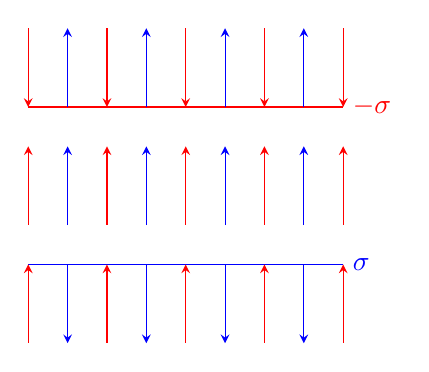
\begin{tikzpicture}
		\def\l{4};
		\def\d{2};
		
		\draw [blue] ({-\l/2}, {-\d/2}) -- ({\l/2}, {-\d/2}) node [right] {$\sigma$};
		\draw [red] ({-\l/2}, {\d/2}) -- ({\l/2}, {\d/2}) node [right] {$-\sigma$};
		
		\begin{scope}[blue, -stealth]
			\foreach \i in {-1.5,...,1.5}
				\draw (\i,{-\d/4}) -- ++(0,1);
		\end{scope}
		
		\begin{scope}[blue, -stealth]
			\foreach \i in {-1.5,...,1.5}
				\draw (\i,{\d/2}) -- ++(0,1);
		\end{scope}
		
		\begin{scope}[blue, -stealth]
			\foreach \i in {-1.5,...,1.5}
				\draw (\i,{-\d/2}) -- ++(0,-1);
		\end{scope}
		
		\begin{scope}[red, stealth-]
			\foreach \i in {-2,...,2}
				\draw (\i,{\d/4}) -- ++(0,-1);
		\end{scope}
		
		\begin{scope}[red, stealth-]
			\foreach \i in {-2,...,2}
				\draw (\i,{\d/2}) -- ++(0,1);
		\end{scope}
		
		\begin{scope}[red, stealth-]
			\foreach \i in {-2,...,2}
				\draw (\i,{-\d/2}) -- ++(0,-1);
		\end{scope}
	\end{tikzpicture}
\end{figure}

The electric field due to the plates are as shown. 
Therefore, the fields between the plates add up and the fields outside the plates cancel out.\\
Therefore, the net field inside the capacitor is 
\begin{equation*}
	{\color{red} \dfrac{\sigma}{2 \varepsilon_0}} + {\color{blue} \dfrac{\sigma}{2 \varepsilon_0}} = \dfrac{\sigma}{\varepsilon_0}
\end{equation*}

\section{Electric Dipoles}

\begin{definition}[Electric dipole]
	Two charges, $q$ and $-q$, separated by a distance $d$ is called an electric dipole.
	\begin{figure}[H]
		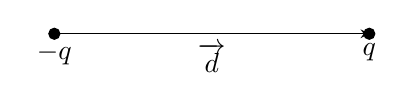
\begin{tikzpicture}
			\def\d{4};
			
			\draw [-stealth] ({-\d/2},0) -- ({\d/2},0) node [midway, below] {$\overrightarrow{d}$};
			
			\filldraw ({-\d/2},0) circle (2pt) node [below] {$-q$};
			\filldraw ({\d/2},0) circle (2pt) node [below] {$q$};
		\end{tikzpicture}
	\end{figure}
\end{definition}

\begin{definition}[Dipole moment]
	If two charges $q$ and $-q$ are separated by a distance $d$, the dipole moment is defined as
	\begin{equation*}
		\overrightarrow{P} \doteq q \cdot \overrightarrow{d}
	\end{equation*}
	where $\overrightarrow{d}$ is the vector of length $d$ pointing from $-q$ to $q$.
\end{definition}

\subsection{Electric Field Due to Electric Dipoles}

\subsubsection{Electric Field}

\begin{figure}[H]
	\begin{tikzpicture}
		\def\d{4};
		\def\x{3};
		
		\coordinate (O) at (0,0);
		\coordinate (+q) at (0,{\d/2});
		\coordinate (-q) at (0,{-\d/2});
		\coordinate (x) at (\x,0);
		
		\begin{scope}[-stealth, lightgray]
			\draw ({-(\x + 1)},0) -- ({\x + 1},0) node [right] {$x$};
			\draw (0,{-(\d/2 + 1)}) -- (0,{\d/2 + 1}) node [above] {$z$};
		\end{scope}
		
		\filldraw (+q) circle (1pt);
		\filldraw (-q) circle (1pt);
		
		\begin{scope}[xshift = -10, |<->|]
			\draw (0,0) -- (0,{\d/2}) node [midway, fill = white] {$\dfrac{d}{2}$};
			\draw (0,0) -- (0,{-\d/2}) node [midway, fill = white] {$\dfrac{d}{2}$};
		\end{scope}
		
		\begin{scope}[dashed, blue]
			\draw (\x,0) -- (+q) node [midway, above right] {$\sqrt{\dfrac{d^2}{4} + z^2}$};
			\draw (\x,0) -- (-q) node [midway, below right] {$\sqrt{\dfrac{d^2}{4} + z^2}$};
		\end{scope}
		
		\begin{scope}[-stealth, blue]
			\draw (\x,0) -- ($ (\x,0) ! -1cm ! (+q) $);
			\draw (\x,0) -- ($ (\x,0) ! 1cm ! (-q) $);
		\end{scope}
		
		\pic [draw,  "$\theta$", angle eccentricity = 1.5] {angle = O--+q--x};
	\end{tikzpicture}
\end{figure}

\begin{align*}
	\overrightarrow{F} &= 2 E_+ \cos \theta (- \hat{z})\\
	&= 2 \cdot \dfrac{1}{4 \pi \varepsilon_0} \dfrac{q}{\left( \dfrac{d}{2} \right)^2 + x^2} \cdot \dfrac{\dfrac{d}{2}}{\left( \left( \dfrac{d}{2} \right)^2 + x^2 \right)^{\sfrac{1}{2}}} (- \hat{z})\\
	&= - \dfrac{1}{4 \pi \varepsilon_0} \dfrac{\overrightarrow{P}}{\left( \left( \dfrac{d}{2} \right)^2 + x^2 \right)^{\sfrac{3}{2}}}
\end{align*}

\section{Gauss' Law}

\begin{definition}[Electric flux]
	Electric flux is defined as the dot product of the electric field passing through a surface, and the area vector of the surface.
	\begin{equation*}
		\Phi = \overrightarrow{E} \cdot \overrightarrow{A}
	\end{equation*}
	where the magnitude of the area vector is proportional to the area of the surface and the direction is perpendicular to the surface.
\end{definition}

This can be modelled as water passing through a surface.

\begin{figure}[H]
	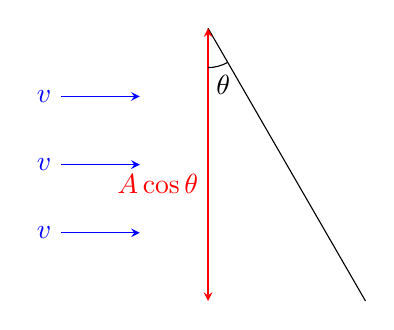
\begin{tikzpicture}
		\def\angle{30};
		\def\l{4};
		
		\coordinate (O) at (0,0);
		\coordinate (plate top) at (0,{\l*cos(\angle)});
		\coordinate (plate bottom) at ($ (plate top) + ({-90 + \angle}:\l) $);
		
		\draw (plate top) -- (plate bottom);
		
		\draw [red, stealth-stealth] (plate top) -- (O) node [midway, below left] {$A \cos \theta$};
		
		\begin{scope}[blue, stealth-]
			\draw ({-\l*cos(\angle)/4},{\l*cos(\angle)/4}) -- ++(180:1) node [left] {$v$};
			\draw ({-\l*cos(\angle)/4},{2*\l*cos(\angle)/4}) -- ++(180:1) node [left] {$v$};
			\draw ({-\l*cos(\angle)/4},{3*\l*cos(\angle)/4}) -- ++(180:1) node [left] {$v$};
		\end{scope}
		
		\pic [draw, "$\theta$", angle eccentricity = 1.5] {angle = O--plate top--plate bottom};
	\end{tikzpicture}
\end{figure}

The flux of the water passing through the area $A$ is $A v \cos \theta$.

\begin{theorem}[Gauss' Law]
	\begin{equation*}
		\oiint \overrightarrow{E} \cdot \overrightarrow{\dif A} = \dfrac{Q_{\textnormal{inside}}}{\varepsilon_0}
	\end{equation*}
\end{theorem}

\begin{question}
	A hollow sphere of radius $R$ has surface charge density $\sigma$. Find the field at a point at distance $r$ from the centre of the sphere.
\end{question}

\begin{solution}
	Consider the imaginary Gaussian surface as a sphere with radius $r$.
	\begin{figure}[H]
		\begin{tikzpicture}
			\def\R{3};
			\def\r{5};
			
			\begin{scope}
				\draw (0,0) circle (\R);
				\draw [dashed] (0,0) -- ++({360*rnd}:\R) node [midway, fill = white] {$R$};
			\end{scope}
			
			\begin{scope}[blue, dashed]
				\draw (0,0) circle (\r);
				\draw [dashed] (0,0) -- ++({360*rnd}:\r) node [midway, fill = white] {$r$};
			\end{scope}
			
		\end{tikzpicture}
	\end{figure}
	Using Gauss' Law over the Gaussian surface,
	\begin{align*}
		\oiint \overrightarrow{E} \cdot \overrightarrow{\dif A} &= \dfrac{Q_{\textnormal{total}}}{\varepsilon_0}\\
		\therefore \oiint E \dif A &= \dfrac{Q_{\textnormal{total}}}{\varepsilon_0}\\
		\therefore E \oiint \dif A &= \dfrac{Q_{\textnormal{total}}}{\varepsilon_0}\\
		\therefore E \cdot 4 \pi r^2 &= \dfrac{Q_{\textnormal{total}}}{\varepsilon_0}\\
		\therefore \overrightarrow{E} &= \dfrac{1}{4 \pi \varepsilon_0} \dfrac{Q_{\textnormal{total}}}{r^2} \hat{r}
	\end{align*}
\end{solution}
~\\
Similarly for $r < R$, $E = 0$.

\section{Electric Potential}

\begin{definition}[Electrical Potential]
	The electric potential due to a point charge $q$ is
	\begin{align*}
		\varphi \left( \overrightarrow{r} \right) &= \dfrac{1}{4 \pi \varepsilon_0} \dfrac{q}{r} + c
	\end{align*}
\end{definition}

If a charge $q$ in moved from point $\textnormal{A}$ to $\textnormal{B}$,
\begin{align*}
	W_{\textnormal{\textnormal{A}} \to \textnormal{B}} &= \int\limits_{\overrightarrow{r_{\textnormal{A}}}}^{\overrightarrow{r_{\textnormal{B}}}} \overrightarrow{E} \cdot \dif \overrightarrow{r}\\
	&= \int\limits_{r_{\textnormal{A}}}^{r_{\textnormal{B}}} \dfrac{1}{4 \pi \varepsilon_0} \dfrac{q}{r^2} \dif r\\
	&= \left. - \dfrac{1}{4 \pi \varepsilon_0} \dfrac{q}{r} \right|_{r_{\textnormal{A}}}^{r_{\textnormal{B}}}\\
	&= \dfrac{1}{4 \pi \varepsilon_0} \dfrac{q}{r_{\textnormal{A}}} - \dfrac{1}{4 \pi \varepsilon_0} \dfrac{q}{r_{\textnormal{B}}}
\end{align*}

Therefore,
\begin{align*}
	W_{\textnormal{A} \to \textnormal{B}} &= \varphi \left( \overrightarrow{r_A} \right) - \varphi \left( \overrightarrow{r_B} \right)\\
	\therefore \varphi \left( \overrightarrow{r_B} - \overrightarrow{r_A} \right) &= - \int\limits_{\overrightarrow{r_A}}^{\overrightarrow{r_B}} \overrightarrow{E} \cdot \dif \overrightarrow{r}
\end{align*}

\begin{question}
	An electric dipole with charges $q$ and $-q$ is placed on the $z$-axis with distance $d$ between the charges.
	Find the field at a general point in space.
	Find points at which the electric potential is zero.
\end{question}

\begin{solution}
	\begin{figure}[H]
		\begin{tikzpicture}
			\def\d{6};
			
			\coordinate (+q) at (0,{\d/2});
			\coordinate (-q) at (0,{-\d/2});
			\coordinate (point) at (\d,0.3*\d);
			
			\begin{scope}[lightgray, -stealth]
			\draw (0,0) -- (5,0) node [right] {$y$};
			\draw (0,0) -- (0,5) node [above] {$z$};
			\end{scope}
			
			\begin{scope}[red, -stealth]
			\draw (0,0) -- (point) node [midway, fill = white] {$r$};
			\draw (+q) -- (point) node [midway, fill = white] {$r_{+}$};
			\draw (-q) -- (point) node [midway, fill = white] {$r_{-}$};
			\end{scope}
			
			\filldraw (+q) circle (2pt) node [left] {$q$};
			\filldraw (-q) circle (2pt) node [left] {$-q$};
		\end{tikzpicture}
	\end{figure}
	Let the electric potential at infinity be zero.
	\begin{align*}
		\varphi \left( \overrightarrow{r} \right) &= \dfrac{1}{4 \pi \varepsilon_0} \left( \dfrac{q}{r_{+}} + \dfrac{-q}{r_{-}} \right)\\
		&= \dfrac{1}{4 \pi \varepsilon_0} \dfrac{q (r_{-} - r_{+})}{r_{-} \cdot r_{+}}
	\end{align*}
	Therefore, the potential is zero only if $r_{+} = r_{-}$.
	Therefore, for all points on the $x y$-plane, the potential is zero.
\end{solution}

\begin{question}
	Find the electric potential at a point at distance $r$ on the equator of a line of charge of length $L$ and uniform line charge density $\lambda$.
\end{question}

\begin{solution}
	Consider an elemental charge $\dif q$ with length $\dif z$ at a distance $z$ from the centre of the line.
	\begin{figure}[H]
		\begin{tikzpicture}
			
		\end{tikzpicture}
	\end{figure}
	\begin{align*}
		\dif q &= \lambda \dif z
	\end{align*}
	Therefore,
	\begin{align*}
		\varphi(r) &= \int \dfrac{1}{4 \pi \varepsilon_0} \dfrac{q}{\sqrt{z^2 + r^2}}\\
		&= \int\limits_{-\sfrac{L}{2}}^{\sfrac{L}{2}} \dfrac{1}{4 \pi \varepsilon_0} \dfrac{\lambda \dif z}{\sqrt{z^2 + r^2}}\\
		&= \dfrac{\lambda}{4 \pi \varepsilon_0} \ln \left( \dfrac{\sqrt{L^2 + 4 r^2} + L}{\sqrt{L^2 + 4 r^2} - L} \right)
	\end{align*}
\end{solution}

\begin{question}
	Find the electric potential due to an infinite line of charge.
\end{question}

\begin{solution}
	For an infinite line of charge, the charge at infinity is not zero.
	Therefore, it is wrong to assume that the electric potential at infinity is zero.
	Therefore, the result for a finite line of charge cannot be used to find the potential due to an infinite line of charge.\\
	Therefore, the potential needs to be calculated using the electric field.
	\begin{align*}
		\varphi(r) - \varphi(r_0) &= -\int\limits_{r_0}^{r} \overrightarrow{E} \cdot \dif \overrightarrow{r}\\
		&= - \int\limits_{r_0}^{r} E \dif r\\
		&= - \int\limits_{r_0}^{r} \dfrac{\lambda}{2 \pi \varepsilon_0 r} \dif r\\
		&= \left. - \dfrac{\lambda}{2 \pi \varepsilon_0} \ln r \right|_{r_0}^{r}\\
		&= \dfrac{\lambda}{2 \pi \varepsilon_0} (\ln r_0 - \ln r)\\
		\therefore \varphi(r) &= \varphi(r_0) + \dfrac{\lambda}{2 \pi \varepsilon_0} (\ln r_0 - \ln r)
	\end{align*}
\end{solution}

\begin{question}
	Find the electric potential due to a hollow sphere with surface charge density $\sigma$ and radius $R$.
\end{question}

\begin{solution}
	Let the electric potential at infinity be zero.\\
	~\\
	\begin{align*}
		\overrightarrow{E} &=
			\begin{cases}
				0 &;\quad r < R\\
				\dfrac{1}{4 \pi \varepsilon_0} \dfrac{q}{r^2} &;\quad r > R\\
			\end{cases}
	\end{align*}
	Therefore, if $r > R$,
	\begin{align*}
		\varphi(r) - \cancelto{0}{\varphi(\infty)} &= - \int\limits_{\infty}^{r} \overrightarrow{E} \cdot \dif \overrightarrow{r}\\
		&= \int\limits_{r}^{\infty} E \dif r\\
		&= \int\limits_{r}^{\infty} \dfrac{1}{4 \pi \varepsilon_0} \dfrac{q}{r^2} \dif r\\
		&= \left. - \dfrac{1}{4 \pi \varepsilon_0} \dfrac{q}{r^2} \right|_{r}^{\infty}\\
		\therefore \varphi(r) &= \dfrac{1}{4 \pi \varepsilon_0} \dfrac{q}{r}
	\end{align*}
	~\\
	If $r < R$,
	\begin{align*}
		\varphi(r) - \varphi(R) &= \int\limits_{R}^{r} \overrightarrow{E} \cdot \dif \overrightarrow{r}\\
		&= \int\limits_{R}^{r} E \dif r\\
		&= \int\limits_{R}^{r} 0 \dif r\\
		\therefore \varphi(r) &= \varphi(R)\\
		&= \dfrac{1}{4 \pi \varepsilon_0} \dfrac{q}{R}
	\end{align*}
	Therefore, the potential is constant.
	~\\
	Therefore,
	\begin{align*}
		\varphi &=
			\begin{cases}
				\dfrac{1}{4 \pi \varepsilon_0} \dfrac{q}{R} &;\quad r \le R\\
				\dfrac{1}{4 \pi \varepsilon_0} \dfrac{q}{r} &;\quad r \ge R\\
			\end{cases}
	\end{align*}
\end{solution}

\begin{question}
	Find the electric potential due a ring of charge with radius $R$ and charge $q$, at a distance $z$ from its centre, on its axis of symmetry.
\end{question}

\begin{solution}
	Let the electric potential at infinity be zero.\\
	~\\
	\begin{align*}
		\varphi_{\textnormal{ring}} &= \int \dfrac{1}{4 \pi \varepsilon_0} \dfrac{\dif q}{r}\\
		&= \int\limits_{0}^{q} \dfrac{1}{4 \pi \varepsilon_0} \dfrac{\dif q}{\sqrt{R^2 + z^2}}\\
		&= \dfrac{1}{4 \pi \varepsilon_0} \dfrac{1}{\sqrt{R^2 + z^2}}
	\end{align*}
\end{solution}

\begin{question}
	Find the electric potential due a disk of charge with radius $R$ and charge $q$, at a distance $z$ from its centre, on its axis of symmetry.
\end{question}

\begin{solution}
	Let the electric potential at infinity be zero.\\
	~\\
	Consider an elemental ring of thickness $\dif r$ and radius $r$.
	Therefore,
	\begin{align*}
		\varphi_{\textnormal{disk}} &= \int \dif \varphi_{\textnormal{ring}}\\
		&= \int \dfrac{1}{4 \pi \varepsilon_0} \dfrac{\dif q_{\textnormal{ring}}}{\sqrt{r^2 + z^2}}\\
		&= \int\limits_{0}^{R} \dfrac{1}{4 \pi \varepsilon_0} \dfrac{2 \pi r \dif r \sigma}{\sqrt{r^2 + z^2}}\\
		&= \dfrac{\sigma}{2 \varepsilon} \left( \sqrt{R^2 + z^2} - |z| \right)
	\end{align*}
\end{solution}

\section{Electrical Potential Energy}

\begin{question}
	Three charges, $q$, $-4q$, $2q$ are placed on the vertices of an equilateral triangle of side $a$. Find the energy in the system.
\end{question}

\begin{solution}
	\begin{figure}[H]
		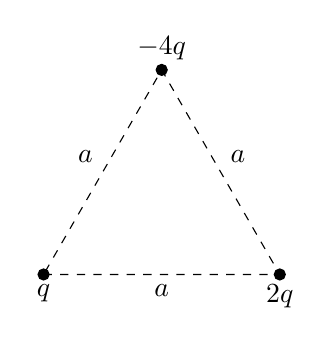
\begin{tikzpicture}
			\def\a{3};
			
			\coordinate (q) at (0,0);
			\coordinate (2q) at (0:\a);
			\coordinate(-4q) at (60:\a);
			
			\filldraw (q) circle (2pt) node [below] {$q$};
			\filldraw (2q) circle (2pt) node [below] {$2q$};
			\filldraw (-4q) circle (2pt) node [above] {$-4q$};
			
			\draw [dashed] (q) -- node [midway, below] {$a$} (2q) -- node [midway, above right] {$a$} (-4q) -- node [midway, above left] {$a$} cycle;
		\end{tikzpicture}
	\end{figure}
	The energy in the system is the amount of energy required to build the system by bringing each of the charges from infinity to its position, one by one.\\
	Let the positions of $q$, $2q$ and $-4q$ be A, B and C respectively.\\
	The energy required to bring the first charge, $q$, from infinity to A is zero, as there are no forces acting on it.\\
	The energy required to bring the second charge, $2q$, from infinity to B is 
	\begin{align*}
		U_{2q} &= - \int\limits_{\infty}^{\overrightarrow{r_\textnormal{B}}} \overrightarrow{F} \cdot \dif \overrightarrow{r}\\
		&= - \int\limits_{\infty}^{\overrightarrow{r_\textnormal{B}}} (2q) \cdot \overrightarrow{E} \cdot \dif \overrightarrow{r}\\
		&= - (2q) \int\limits_{\infty}^{\overrightarrow{r_\textnormal{B}}} \overrightarrow{E} \cdot \dif \overrightarrow{r}\\
		&= (2q) \left( \varphi(\textnormal{B}) - \varphi(\infty) \right)\\
		&= (2q) \cdot \varphi(\textnormal{B})
	\end{align*}
	where $\varphi(\textnormal{B})$ is potential at point B due to the existing charges, i.e. $q$.
	Similarly, the energy required to bring the third charge, $-4q$, from infinity to C is $(-4q) \cdot \varphi(\textnormal{C})$, where $\varphi(\textnormal{C})$ is the potential at point C due to the existing charges, i.e. $q$ and $2q$.\\
	Therefore, the total energy required is
	\begin{align*}
		U &= \left( 0 \right) + (2q) \left( \dfrac{1}{4 \pi \varepsilon_0} \dfrac{q}{a^2} \right) + (-4q) \left( \dfrac{1}{4 \pi \varepsilon_0} \dfrac{q}{a^2} + \dfrac{1}{4 \pi \varepsilon_0} \dfrac{2q}{a^2} \right)
	\end{align*}
\end{solution}

\begin{question}
	Find the potential energy in a solid sphere of charge, with charge density $\rho$ and radius $R$.
\end{question}

\begin{solution}
	Consider a solid sphere of charge with $\rho$ and $r$.
	Consider an elemental shell of thickness $\dif r$ on this sphere.\\
	Therefore,
	\begin{align*}
		\dif V &= 4 \pi r^2 \dif r\\
		\therefore \dif q &= \rho \cdot \dif V\\
		&= 4 \pi \rho r^2 \dif r
	\end{align*}
	Therefore,
	\begin{align*}
		\dif U &= \dfrac{1}{4 \pi \varepsilon_0} \dfrac{q_{\textnormal{inside}}}{r} \dif q\\
		&= \dfrac{1}{4 \pi \varepsilon_0} \dfrac{\dfrac{4}{3} \pi r^3 \rho}{r} \cdot 4 \pi r^2 \dif r \rho\\
		\therefore U &= \int\limits_{0}^{R} \dfrac{4 \pi \rho^2}{3 \varepsilon_0} r^4 \dif r\\
		&= \dfrac{4 \pi \rho^2 R^5}{15 \varepsilon_0}
	\end{align*}
\end{solution}

\section{Integral Form of Gauss' Law}

The volume of the elemental body used for integration is denoted by $\dif^3 r$.\\
For Cartesian coordinate systems, $\dif^3 r = \dif x \dif y \dif z$.\\
For cylindrical coordinate systems, $\dif^3 r = r \dif \theta \dif \varphi \dif z$.\\
For spherical coordinate systems, $\dif^3 r = r^2 \sin \theta \dif r \dif \theta \dif \varphi $.\\

\begin{align*}
	\iint\limits_{\partial V} \overrightarrow{E} \cdot \dif \overrightarrow{A} &= \dfrac{1}{\varepsilon_0} Q_{\textnormal{inside}}\\
	&= \dfrac{1}{\varepsilon_0} \iiint\limits_{V} \rho \dif^3 r 
	\footnotemark
\end{align*}

If a body with volume $V$ and surface area $S$ is cut into two parts, with volumes $V_1$ and $V_2$ and surface area $S_1$ and $S_2$ respectively,
\begin{equation*}
	V = V_1 + V_2
\end{equation*}
However, the surface area increases,
\begin{equation*}
	S = S_1 + S_2 + 2 A \neq S_1 + S_2
\end{equation*}
where $A$ is the area of the new surface created due to the cut.\\
Therefore,
\begin{align*}
	\iint\limits_{S_1} \overrightarrow{E} \cdot \dif \overrightarrow{A} + \iint\limits_{S_2} \overrightarrow{E} \cdot \dif \overrightarrow{A} &= \iint\limits_{\partial V} \overrightarrow{E} \cdot \dif \overrightarrow{A}
\end{align*}

Consider a small cuboid of sides $\dif x$, $\dif y$, $\dif z$.
Let the vertex of the cube, nearest to the origin be $(x,y,z)$.\\
Therefore,
\begin{align*}
	\Phi &= \quad E_z \left( x + \dfrac{\dif x}{2}, y + \dfrac{\dif y}{2}, z + \dif z \right) \dif x \dif y\\
	&\quad - E_z \left( x + \dfrac{\dif x}{2}, y + \dfrac{\dif y}{2}, z \right) \dif x \dif y\\
	&\quad + E_y \left( x + \dfrac{\dif x}{2}, y + \dif y, z + \dfrac{\dif z}{2} \right) \dif x \dif z\\
	&\quad  - E_y \left( x + \dfrac{\dif x}{2}, y, z + \dfrac{\dif z}{2} \right) \dif x \dif z\\
	&\quad + E_x \left( x + \dif x, y + \dfrac{\dif y}{2}, z + \dfrac{\dif z}{2} \right) \dif y \dif z\\
	&\quad  - E_x \left( x, y + \dfrac{\dif y}{2}, z + \dfrac{\dif z}{2} \right) \dif y \dif z\\
	&= \quad \dfrac{E_z \left( x + \dfrac{\dif x}{2}, y + \dfrac{\dif y}{2}, z + \dif z \right) - E_z \left( x + \dfrac{\dif x}{2}, y + \dfrac{\dif y}{2}, z \right)}{\dif z} \dif x \dif y\\
	&\quad + \dfrac{E_y \left( x + \dfrac{\dif x}{2}, y + \dif y, z + \dfrac{\dif z}{2} \right) - E_y \left( x + \dfrac{\dif x}{2}, y, z + \dfrac{\dif z}{2} \right)}{\dif y} \dif x \dif z\\
	&\quad + \dfrac{E_x \left( x + \dif x, y + \dfrac{\dif y}{2}, z + \dfrac{\dif z}{2} \right) - E_x \left( x, y + \dfrac{\dif y}{2}, z + \dfrac{\dif z}{2} \right)}{\dif x} \dif y \dif z\\
	&= \quad \left( \left. \dpd{E_x}{x} \right|_{\left( x + \frac{\dif x}{2}, y + \frac{\dif y}{2}, z \right)} \right.\\
	&\quad \quad + \left. \dpd{E_y}{y} \right|_{\left( x + \frac{\dif x}{2}, y, z + \frac{\dif z}{2} \right)}\\
	&\quad \quad + \left. \left. \dpd{E_z}{z} \right|_{\left( x + \frac{\dif x}{2}, y + \frac{\dif y}{2}, z \right)} \right) \dif x \dif y \dif z\\
\end{align*}
Therefore
\begin{align*}
	\divergence \overrightarrow{E} &= \lim\limits_{\dif x \to 0, \dif y \to 0, \dif z \to 0} \dfrac{\Phi}{\dif x \dif y \dif z}\\
	&= \left. \left( \dpd{E_x}{x} + \dpd{E_y}{y} + \dpd{E_z}{z} \right) \right|_{(x,y,z)}\\
	&= \overrightarrow{\nabla} \cdot \overrightarrow{E}
\end{align*}

\begin{align*}
	\overrightarrow{E} &= -\overrightarrow{\nabla} \varphi\\
	\therefore \divergence \overrightarrow{E} &= \overrightarrow{\nabla} \cdot \left( -\overrightarrow{\nabla} \varphi \right)\\
	&= \dpd[2]{\varphi}{x} + \dpd[2]{\varphi}{y} + \dpd[2]{\varphi}{x}\\
	&= \nabla^2 \varphi = \Delta \varphi
\end{align*}

\begin{definition}[Laplacian]
	$\nabla^2$ is called the Laplacian.
\end{definition}

\section{Vector Analyses in Cylindrical and Spherical Coordinate Systems}

\subsection{Cylindrical Coordinates}

\begin{align*}
	\overrightarrow{\nabla} f &= \dpd{f}{r} \hat{r} + \dfrac{1}{r} \dpd{f}{\theta} \hat{\theta} + \dpd{f}{z} \hat{z}\\
	\overrightarrow{\nabla} \cdot \overrightarrow{F} &= \dfrac{1}{r} \dpd{}{r} (r F_r) + \dfrac{1}{r} \dpd{F_{\theta}}{\theta} + \dpd{F_z}{z}\\
	\overrightarrow{\nabla} \times \overrightarrow{F} &= \left( \dfrac{1}{r} \dpd{F_z}{\theta} - \dpd{F_{\theta}}{z} \right) \hat{r} + \left( \dpd{F_r}{z} - \dpd{F_z}{r} \right) \hat{\theta} + \dfrac{1}{r} \left( \dpd{}{r} (r F_{\theta}) - \dpd{F_r}{\theta} \right) \hat{z}\\
	\nabla^2 f &= \dfrac{1}{r} \dpd{}{r} \left( r \dpd{f}{r} \right) + \dfrac{1}{r^2} \dpd[2]{f}{\theta} + \dpd[2]{f}{z}
\end{align*}

\subsection{Spherical Coordinates}

\begin{align*}
	\overrightarrow{\nabla} f &= \dpd{f}{r} \hat{r} + \dfrac{1}{r} \dpd{f}{\theta} \hat{\theta} + \dfrac{1}{r \sin \theta} \dpd{f}{\varphi} \hat{\varphi}\\
	\overrightarrow{\nabla} \cdot \overrightarrow{F} &= \dfrac{1}{r^2} \dpd{}{r} (r^2 F_r) + \dfrac{1}{r \sin \theta} \dpd{}{\theta} (F_{\theta} \sin \theta) + \dfrac{1}{r \sin \theta} \dpd{F_{\varphi}}{f}\\
	\overrightarrow{\nabla} \times \overrightarrow{F} &= \quad \dfrac{1}{r \sin \theta} \left( \dpd{}{\theta} (F_{\varphi} \sin \theta) - \dpd{F_{\theta}}{\varphi} \right) \hat{r}\\
	&\quad + \dfrac{1}{r} \left( \dfrac{1}{\sin \theta} \dpd{F_r}{\varphi} - \dpd{}{r} (r F_{\varphi}) \right) \hat{\theta}\\
	&\quad + \dfrac{1}{r} \left( \dpd{}{r} (r F_{\theta}) - \dpd{F_r}{\theta} \right) \hat{\varphi}\\
	\nabla^2 f &= \dfrac{1}{r^2} \dpd{}{r} \left( r^2 \dpd{f}{r} \right) + \dfrac{1}{r^2 \sin \theta} \dpd{}{\theta} \left( \sin \theta \dpd{f}{\theta} \right) + \dfrac{1}{r^2 \sin^2 \theta} \dpd[2]{f}{\varphi}
\end{align*}

\section{Conductors}

In an electrostatic condition, the field inside a conductor is zero.
If it is not, as the conductor allows movement of charged particles, there will be a current and the condition will not be electrostatic.

\begin{question}
	A point charge $q$ is kept inside a cavity in a conducting sphere.
	Find the charge on the surfaces of the sphere.
	\begin{figure}[H]
		\begin{tikzpicture}
			\def\R{3};

			\coordinate (cavity centre) at ({(\R/4)*rand()},{(\R/4)*rand()});

			\draw (0,0) circle (\R);
			\draw (cavity centre) circle (\R/4);

			\fill (cavity centre) circle (2pt) node [left] {$q$};
		\end{tikzpicture}
	\end{figure}
\end{question}

\begin{solution}
	As the sphere is neutral, $\varphi = 0$.\\
	Therefore, $-\dfrac{\rho}{\varepsilon_0} = 0$.\\
	Therefore, by the Poisson equation,
	\begin{align*}
		\nabla^2 \varphi &= 0\\
		\therefore \dfrac{1}{r^2} \dpd{}{r} \left( r^2 \dpd{\varphi}{r} \right) &= 0\\
		\therefore \dpd{}{r} \left( r^2 \dpd{\varphi}{r} \right) &= 0\\
		\therefore r^2 \dpd{\varphi}{r} &= c\\
		\therefore \dpd{\varphi}{r} &= \dfrac{c}{r^2}\\
		\therefore \varphi &= \int \dfrac{c}{r^2} \dif r\\
		&= -\dfrac{c}{r} + d\\
		\intertext{As $\varphi(\infty) = 0$, $d = 0$. Therefore,}
		\varphi &= -\dfrac{c}{r}
	\end{align*}
	Therefore,
	\begin{align*}
		\varphi(R) = -\dfrac{c}{R}\\
		\therefore c &= -R \varphi(R)\\
		\therefore \overrightarrow{E} &= -\overrightarrow{\nabla} \varphi(r)\\
		&= -\dpd{\varphi}{r} \hat{r}\\
		&= -\left( -\dfrac{R \varphi(R)}{r^2} \right) \hat{r}\\
		&= \dfrac{R \varphi(R)}{r^2} \hat{r}
	\end{align*}
	Therefore, the field is constant all over the outer surface.\\
	Therefore, 
	\begin{align*}
		\therefore \sigma &= \dfrac{q}{4 \pi R^2}
	\end{align*}
\end{solution}

\section{Capacitors}

A capacitor is constructed by arranging two conductors, charged with opposite charges.\\
Suppose the charges on the conductors are $+Q$ and $-Q$.
Therefore,
\begin{align*}
	V &= \varphi(+) - \varphi(-)\\
	&= -\int\limits_{(-)}^{(+)} \overrightarrow{E} \cdot \dif \overrightarrow{l}\\
	&= \int\limits_{(+)}^{(-)} \overrightarrow{E} \cdot \dif \overrightarrow{l}\\
	\therefore V &\propto Q
\end{align*}

\begin{definition}[Capacitance]
	Let the charges on the opposite terminals of a capacitor be $+Q$ and $-Q$ respectively.
	The ratio between $Q$ and the potential difference between the terminals is called the capacitance of the capacitor.
	\begin{equation*}
		C = \dfrac{Q}{V}
	\end{equation*}
\end{definition}

\subsection{Parallel Plate Capacitors}

Consider a capacitor made of two conducting plates of surface area $A$ each.
Let the distance between them be $d$.
Let the charge distribution on the plates be $\sigma$ and $-\sigma$ respectively.\\
\begin{figure}[H]
	\begin{tikzpicture}
		\def\d{1};
		\def\l{3};

		\def\xMIN{-\l/2 - 1};
		\def\xMAX{\l/2 + 1};

		\def\yMIN{-1};
		\def\yMAX{\d + 1};

		\begin{scope}[lightgray, stealth-stealth]
			\draw (\xMIN,0) -- (\xMAX,0) node [right] {$y$};
			\draw (0,\yMIN) -- (0,\yMAX) node [above] {$z$};
		\end{scope}

		\begin{scope}[thick]
			\draw ({-\l/2},0) -- ({\l/2},0);
			\draw ({-\l/2},\d) -- ({\l/2},\d);
		\end{scope}
	\end{tikzpicture}
\end{figure}
If $d$ is very small compared to $A$, the plates can be considered to be infinite.\\
Therefore,
\begin{equation*}
	\overrightarrow{E} = 
		\begin{cases}
			\dfrac{\sigma}{\varepsilon_0} \hat{z} &;\quad 0 < z < d\\
			0                                     &;\quad z < 0 \text{ or } z > d\\
		\end{cases}
\end{equation*}
Therefore,
\begin{align*}
	C &= \dfrac{Q}{V}\\
	  &= \dfrac{\sigma A}{E d}\\
	  &= \dfrac{\sigma A}{\dfrac{\sigma}{\varepsilon_0} \cdot d}\\
	  &= \dfrac{A \varepsilon_0}{d}
\end{align*}

\subsection{Concentric Spherical Capacitor}

Consider a conducting sphere, with radius $R_1$ and charge $+Q$, surrounded by a concentric conducting shell of radius $R_2$ and charge $-Q$.
Therefore, the potential difference between the any point at $R_1$ from the centre and any point at $R_2$ from the centre is
\begin{align*}
	           V &= \varphi(R_1) - \varphi(R_2)\\
	             &= -\int\limits_{R_2}^{R_1} \overrightarrow{E} \cdot \dif \overrightarrow{r}\\
	             &= \int\limits_{R_1}^{R_2} \overrightarrow{E} \cdot \dif \overrightarrow{r}\\
	             &= \int\limits_{R_1}^{R_2} E \dif r\\
	             &= \int\limits_{R_1}^{R_2} \dfrac{Q}{4 \pi \varepsilon_0 r^2} \dif r\\
	             &= \left. -\dfrac{Q}{4 \pi \varepsilon_0 r} \right|_{R_1}^{R_2}\\
	             &= \dfrac{Q}{4 \pi \varepsilon_0} \left( \dfrac{1}{R_1} - \dfrac{1}{R_2} \right)\\
	\therefore C &= \dfrac{Q}{V}\\
	             &= \dfrac{4 \pi \varepsilon_0}{\dfrac{1}{R_1} - \dfrac{1}{R_2}}\\
	             &= 4 \pi \varepsilon_0 \dfrac{R_1 R_2}{R_2 - R_1}
\end{align*}

\subsection{Capacitors in Series}

\begin{figure}[H]
	\begin{circuitikz}
		\draw 
			(0,0) to             (1,0)
			(1,0) to [C = $C_1$] (3,0)
			(3,0) to             (4,0)
			(4,0) to [C = $C_2$] (6,0)
			(6,0) to             (7,0);

		\node [below left] at (2,0) {$+Q$};
		\node [below right] at (2,0) {$-Q$};
		\node [below left] at (5,0) {$+Q$};
		\node [below right] at (5,0) {$-Q$};

		\node [left] at (0,0) {$\varphi_A$};
		\node [right] at (7,0) {$\varphi_B$};
		\node [above] at (3.5,0) {$\varphi_C$};
	\end{circuitikz}
\end{figure}

\begin{align*}
	           V                              &= (\varphi_A - \varphi_C) + (\varphi_C - \varphi_B)\\
	                                          &= \dfrac{Q}{C_1} + \dfrac{Q}{C_2}\\
	\therefore \dfrac{Q}{C_{\textnormal{eq}}} &= \dfrac{Q}{C_1} + \dfrac{Q}{C_2}\\
	\therefore \dfrac{1}{C_{\textnormal{eq}}} &= \dfrac{1}{C_1} + \dfrac{1}{C_2}
\end{align*}

\subsection{Capacitors in Parallel}

\begin{align*}
	C_{\textnormal{eq}} &= C_1 +C_2
\end{align*}

\subsection{Energy Stored in a Capacitor}

Consider a capacitor with potential difference $V$ and charge $Q$.\\
The energy required to move an elemental charge $\dif q$ from the negatively charged plate to the positively charged plate is
\begin{align*}
	           \dif U &= V \dif q\\
	                  &= \dfrac{q}{C} \dif q\\
	\therefore U      &= \int\limits_{0}^{Q} \dfrac{q}{C} \dif q\\
	                  &= \dfrac{Q^2}{2 C}\\
			  &= \dfrac{1}{2} Q V\\
			  &= \dfrac{1}{2} C V^2
\end{align*}

\end{document}
